\documentclass[11pt]{report}
\usepackage{outline}
\usepackage[sfdefault]{roboto}
\usepackage{pmgraph}
\usepackage[normalem]{ulem}
\usepackage{listings}
\usepackage{geometry}
\usepackage{float}
\usepackage{longtable}
\usepackage{graphicx}
\graphicspath{{Figures/}}
\lstset{language = SQL, breaklines=true}
\title{\textbf{System Maintenance}}
\author{Thomas Moffat, 51337, 4042}
\setlength{\oddsidemargin}{0in}
\setlength{\evensidemargin}{0in}
\setlength{\topmargin}{0in}
\setlength{\headsep}{-.25in}
\setlength{\textwidth}{6.5in}
\setlength{\textheight}{8.5in}
%--------------------Indention
\setlength{\parindent}{1cm}

\begin{document}
%--------------------Title Page
\maketitle

\section{System Overview}
This is a system designed for a small swimming club to allow them to remove the current paper based system for ordering kit and instead go entirely paper-less. This system allows customers to place orders using a web form which is then passed into a database, and then allows the Kit Coordinator to view all of these entries, as well as generate the order form for the suppliers. The system retains the customer details for future reference, if people need to know what they ordered previously. \par A new customer can be created by the customer accessing the order form and filling in their details (string/int) which is then passed to a MySQL database. A new item order is created by them submitting their details and then redirecting to the next page, filling in the order form there and submitting it. This is again passed to the MySQL database. A new connection is created by calling the getConnection function in the Java program, which gets the connection details from kitorder.xml, and then Driver\_Manager to create a connection to the database. The search function in the Java program gets the search string (string) typed in from the MainMenu and the order (string) and inputs these into an SQL statement with wildcards, returning the ResultSet as part of a dynamic JavaFX TableView. This is also how the TableView function works, just lacking the search string. To generate an order form, a Python script is called from the Java code, which then connects to the database, retrieves the relevant details for each item as a ResultSet and then inputs them into the spreadsheet using openpyxl, which can then be sent to the printers. In this, each item has its own sheet for clarity. The final non-trivial process in this program is the database dump feature, which makes a backup of the contents of the database in CSV files, then calls Mybatis, which executes a SQL script, dropping all of the tables in the database and then recreating them as new blank tables. Following this it calls a CSVReader function which reads a CSV file to recreate the items table of the database, as this never needs to change. \par This program is connected to a MySQL database. The Customer, Order and Items are stored in separate, related tables which use foreign keys to ensure accuracy of data. When a new order is created, an appropriate SQL statement is generated and the order is inserted into the database. 
\section{Algorithms}
	Due to the nature of the code, for reasons explained Section 2.6 of the main report, there are no data manipulation algorithms in this report, although there are four quite complex SQL statements that are used in the program. They  are given as follows, and discussed:
\begin{lstlisting}
	select o . ID , o . Orders , o . CustomerID , c .Name, c . Email_Address , c . Squad , o . OrderSize , o . OrderNumber , o . PaymentMethod , i . Item from INNER JOIN Items i ON i.idItems=o.Order where o.ID like ? or o.CustomerID like ? or c.Name like ? or c.Email_Address like ? or c. Squad like ? or o.Orders like ? or o.OrderSize like ? or o.OrderNumber like ? or o.NameOnGarment like ? or o. PaymentMethod like ? or i . Item like ? ORDER BY ?;	
\end{lstlisting}
This is the search algorithm for the DBSearch.java function. This is set up as a prepared statement so that a SQL injection is impossible to undertake. Each of the question marks in this case represents the same thing, the search string. In the Java code this has \% appended to the beginning and end to act as wild cards. The source code for this is as follows: 
\lstinputlisting[linerange=50-89, language=java, numbers=left, numberstyle=\tiny, stepnumber=1, numbersep=5pt]{/Users/tsmoffat/kitordersystem/kitordersystem/kitordersystem/DBSearch.java}
This code also shows how the program deals with setting the ordering, i.e. it takes a variable from the MainMenu and uses a switch case to convert it into a form that MySQL will understand. However the important bit is lines 30-40, where the input is mapped to each of the question marks in the SQL statement in order. This allows the user to put in anything, even a SQL statement and absolutely nothing will happen, as the special characters in the statement are being ignored and so are inserted into the database verbatim. 
\par
	The next SQL statement is very similar to the previous one, it just doesn't have any of the prepared statement as it doesn't take directly user-editable inputs. This means that it takes a value selectable from a drop-down menu and uses that to order the results, but the user can't put their own string in its place. It goes thusly:
\begin{lstlisting}
	select o.ID, o.CustomerID, c.Name, c.Email_Address, c.Squad, o.Orders, o.OrderSize, o.OrderNumber, o.NameOnGarment, o.PaidFor, o.PaymentMethod, i.Item from Orders o INNER JOIN Customers c ON o.CustomerID = c.ID INNER JOIN Items i ON i.idItems=o.Order ORDER BY ?;	
\end{lstlisting}
The code for how this part of the program deals with ordering is exactly the same as the previous one. \par 
The third SQL statement is called when the database is remade. This dumps the contents of the Customers and Orders tables into two CSV  files which can then be used for further reference or to repopulate the database after it has been wiped clean. It follows as such:
\begin{lstlisting}
	SELECT * FROM Customers INTO OUTFILE /Users/tsmoffat/kitordersystem/kitordersystem/kitordersystem/Customers.csv FIELDS ENCLOSED BY '"' TERMINATED BY ';' ESCAPED BY '"' LINES TERMINATED BY '\r\n'; SELECT * FROM Orders INTO OUTFILE /Users/tsmoffat/kitordersystem/kitordersystem/kitordersystem/Orders.csv FIELDS ENCLOSED BY '"' TERMINATED BY ';' ESCAPED BY '"' LINES TERMINATED BY '\r\n';
\end{lstlisting}
This statement is actually two almost identical statements acting one after the other. First everything is taken from the Customers table and put into a CSV file where each item is enclosed with "", each line is finished with a semi-colon and then a carriage return is performed to input the next row of data. This is exactly the same with the second statement except that takes all the values from the orders table.\par The final complex SQL statement is actually a script, which is called when the database is reset. This drops every table in the database then remakes them blank. It is given here:
\lstinputlisting[numbers=left, numberstyle=\tiny, stepnumber=1, numbersep=5pt]{/Users/tsmoffat/kitordersystem/kitordersystem/kitordersystem/KitOrderProper.sql}
This is obviously a very long series of statements but we shall go through the important parts one by one. To begin with, it tells MySQL to drop the Customers table and then create again, with all the columns remade, with ID auto-incrementing, the length of Squad, Name and Email\_Address set to 45 and set to not be null, then sets the primary key and the unique index. Following this it repeats the process with the Items table. Then the orders table undergoes the same process, with a couple of differences. As this is the primary table of this database, it has a couple of foreign keys, the item ID from  the items table and the customer ID from the Customers table. This is for a bit of error checking, so that no orders can point to a customer or item that don't exist, which would obviously create some errors. 
\newgeometry{left=1.25cm}
\section{Procedure and Variable Lists}
	
		\begin{longtable}{|p{0.2\linewidth}|p{0.8\linewidth}|}
			\caption{Procedure Listings}\\
			\hline 
			Procedure & Description\\[0.5ex]
			\hline
			\endhead
			\hline
			\endfoot
			MainMenu & Shows the main menu of the program, allows every other function in the program to be called in one way or another \\
			getConnection & Opens a connection to the database\\
			SetProperties & Sets the properties of the connection from kitorder.xml that is used by getConnection\\
			DBReset & Resets the database after pulling all of the contents of the database to CSV files\\
			CSVReader & Reads the CSV file that contains the data for the items table and inserts it into said table after a reset \\
			TableViewTest & Shows all of the database contents \\
			DBSearch & Same as TableViewTest except this also takes a search string \\
			DocWriter & Calls a python script to output the relevant contents of the database to an Excel file \\
			docdump & Python script that outputs all of the contents of the database to an Excel file \\
			dbcustomerupdate & Takes the values from the HTML customer page and inserts them into the database \\
			dborderupdate & Takes the values from the order form and inserts them into the database \\
			WebInputpasstophp & Passes the values from the HTML customer details form to the PHP script via post, then redirects to the order page \\
			WebOrderInput passtophp & Passes the values from the HTML to the dborderupdate PHP script\\
		\end{longtable}	
	\begin{longtable}{|p{0.2\linewidth}|p{0.2\linewidth}|p{0.2\linewidth}|p{0.2\linewidth}|p{0.2\linewidth}|}
			\caption{Variable Listing}\\
			\hline
			Procedure & Global/Local Variable & Variable Name & Data Type & Description \\[0.5ex]
			\hline
			\endhead
			\hline
			\endfoot
			MainMenu & Global & token & String & Stores the search token for the DBSearch class\\
			 & Global & ordering & String & Stores the ordering for the DBSearch and TableViewTest classes\\
			 & Local & remakeButton & Button & Creates a button instance\\
			 & Local & dbViewButton & Button & Creates a button instance\\
			 & Local & emailButton & Button & Creates a button instance\\
			 & Local & searchButton & Button & Creates a button instance\\
			 & Local & searchField & TextField & Creates a text field instance\\
			 & Local & orderComboBox & ComboBox & Creates a combo box instance\\
			 & Local & label & Label & Creates a label instance\\
			 & Local & dialog & TextInputDialog & Creates a text input dialog instance \\
			 & Local & result & Optional <String> & Stores the input result from dialog\\
			 & Local & result1 & String & Stores result as a string \\
			 & Local & reset & DBReset & Creates a new DBReset instance\\
			 & Local & reader & CSVReader & creates a new CSVReader instance \\
			 & Local & e & One of a number of exceptions & stores the exception thrown \\
			 & Local & alert & Alert & Creates a new dialog box\\
			 & Local & sw & StringWriter & writes a stack trace to a string \\
			 & Local & pw & PrintWriter & prints stack trace to pw \\
			 & Local & textArea & TextArea & creates a new TextArea \\
			 & Local & expContent & GridPane & creates a new GridPane\\
			 & Local & writer & DocWriter & Calls a new instance of the DocWriter class \\
			 & Local & grid & GridPane & Creates a new GridPane instance\\
			 & Local & scene & Scene & Creates a new scene \\
			 \hline
			getConnection & Global & dbms & String & Stores the dbms\\
			 & Global & dbName & String & Stores the database name \\
			 & Global & userName & String & Stores the username for the database\\
			 & Global & password & String & Stores the password for the database\\
			 & Global & portNumber & private int & Stores the port number to access the database \\
			 & Local & conn & Connection & stores the connection to the database \\
			 & Local & dbFactory & DocumentBuilder Factory & Creates a new instance of a documentbuilderfactory \\
			 & Local & dBuilder & DocumentBuilder & Creates a new DocumentBuilder instance \\
			 & Local & doc & Document & Creates a new document instance \\
			 & Local & nList & NodeList & Creates a new node list to store XML \\
			 & Local & database & Element & Stores the database element from the XML file\\
			\hline
			DBReset & Local & SQLFilePath & String & Stores the file path to the SQL script \\
			 & Local & sqlExport & String & Stores the SQL command to output the contents of the database file to CSV files \\
			 & Local & conn & Connection & Stores a connection from getConnection\\
			 & Local & sr & ScriptRunner & Creates a new ScriptRunner instance \\
			 & Local & reader & Reader & Creates a new reader that reads the file from SQLFilePath \\
			 & Local & e & One of a number of exceptions & stores the exception thrown \\
			 & Local & alert & Alert & Creates a new dialog box\\
			 & Local & sw & StringWriter & writes a stack trace to a string \\
			 & Local & pw & PrintWriter & prints stack trace to pw \\
			 & Local & textArea & TextArea & creates a new TextArea \\
			 & Local & expContent & GridPane & creates a new GridPane\\
			 \hline
			CSVReader & Local & reader & BufferedReader & Creates a new reader to read a CSV file \\
			 & Local & c & Connection & Gets a connection from getConnection\\
			 & Local & st & Statement & Creates a SQL statement \\
			 & Local & line & String & Stores the current line of the CSV\\
			 & Local & item & String[] & Stores the contents of the current line as an array\\
			 \hline
			TableViewTest & Global & tableview & TableView & Creates a new tableview instance\\
			 & Local & c & Connection & Stores connection\\
			 & Local & data & ObservableList<ObservableList> & Creates a new list of type ObservableList<ObservableList> \\
			 & Local & SQL & String & Stores SQL statements \\
			 & Local & ordering & String & Stores the ordering from the main menu \\
			 & Local & order & String & Stores the ordering in a MySQL-friendly format \\
			 & Local & rs & ResultSet & Creates a new ResultSet to store data from the database in \\
			 & Local & col & TableColumn & Creates a new TableColumn \\
			 & Local & row  & ObservableList <String> & Creates a new list of type ObservableList<String> \\
			 & Local & e & One of a number of exceptions & stores the exception thrown \\
			 & Local & alert & Alert & Creates a new dialog box\\
			 & Local & sw & StringWriter & writes a stack trace to a string \\
			 & Local & pw & PrintWriter & prints stack trace to pw \\
			 & Local & textArea & TextArea & creates a new TextArea \\
			 & Local & expContent & GridPane & creates a new GridPane\\
			 \hline
			DBSearch & Local & data & ObservableList <ObservableList> & Creates a new list of type ObservableList <ObservableList> \\
			 & Local & c & Connection & Stores connection\\
			 & Local & SQL & String & Stores SQL statements \\
			 & Local & token & String & Stores the search string from the main menu \\
			 & Local & ordering & String & Stores the ordering from the main menu \\
			 & Local & order & String & Stores the ordering in a MySQL-friendly format \\
			 & Local & rs & ResultSet & Creates a new ResultSet to store data from the database in \\
			 & Local & col & TableColumn & Creates a new TableColumn \\
			 & Local & row  & ObservableList <String> & Creates a new list of type ObservableList <String> \\
			 & Local & e & One of a number of exceptions & stores the exception thrown \\
			 & Local & alert & Alert & Creates a new dialog box\\
			 & Local & sw & StringWriter & writes a stack trace to a string \\
			 & Local & pw & PrintWriter & prints stack trace to pw \\
			 & Local & textArea & TextArea & creates a new TextArea \\
			 & Local & expContent & GridPane & creates a new GridPane\\ 
			\hline
			DocWriter & Local & pythonScriptPath & String & Stores the path to the python script \\
			 & Local & cmd & String[] & An array that stores details to execute the python script \\
			 & Local & rt & Runtime & Creates a new runtime \\
			 & Local & pr & Process & Creates a new process \\
			 \hline
			docdump & Local & tree & ElementTree & Stores the whole XML tree \\
			 & Local & root & ElementTree & Gets the root element of tree \\
			 & Local & dbms & String & Gets the dbms from the root \\
			 & Local & database\_name & String & Gets the database name from the root \\
			 & Local & user\_name & String & Gets the username from the root \\
			 & Local & password & String & Gets the password from the root \\
			 & Local & port\_number & String & Gets the port number from the root \\
			 & Local & server\_name & String & Gets the server IP address from the root \\
			 & Local & db & Connection & Gets a connection to the database \\
			 & Local & cur & Cursor & Creates a cursor to navigate the database \\
			 & Local & wb & Workbook & Creates a new Excel workbook \\
			 & Local & ws1 & Worksheet & Creates a new worksheet in the workbook\\
			 & Local & x & int & Stores how many times the cycle has been iterated through\\
			 & Local & xstring & String & Stores x in a string\\
			 & Local & item & String & Stores the current item \\
			 & Local & row & Row & Stores the current row from the resultset \\
			 & Local & d & Cell & Stores a cell \\
			 & Local & e & Cell & Stores a cell \\
			 & Local & f & Cell & Stores a cell \\
			 & Local & i & int & Stores which row the pointer is on \\
			\hline
			dbcustomerupdate & Local & \$xml & simplexml & Stores XML tree\\
			 & Local & \$dbms & String & Stores dbms from XML \\
			 & Local & \$dbname & String & Stores database name from XML \\
			 & Local & \$user\_name & String & Stores username from XML \\
			 & Local & \$password & String & Stores password from XML \\
			 & Local & \$port\_numberraw & String & Stores the string port number from XML \\
			 & Local & \$port\_number & int & Stores the port number as an int \\
			 & Local & \$servername & String & Stores server IP address from XML \\
			 & Local & \$conn & Connection & Stores connection to the database \\
			 &  Local & \$name & String & Stores name from web form \\ 
			 &  Local & \$email & String & Stores email from web form \\ 
			 &  Local & \$squad & String & Stores squad from web form \\
			 &  Local & \$paymethod & String & Stores payment method from web form \\
			 & Global & \$\_SESSION ["paymethod"] & String & Stores paymethod as a Session variable \\
			 & Local & \$stmt & SQL Statement & Stores SQL statement to be executed \\
			 & local & \$sql & SQL Statement & Stores SQL statement to be executed \\
			 & Local & \$result & String & Stores user ID \\
			 & Global & \$\_SESSION["ID"] & String & Stores User ID as a global variable \\
			 \hline
			DBOrderUpdate & Local & \$xml & simplexml & Stores XML tree\\
			& Local & \$dbms & String & Stores dbms from XML \\
			 & Local & \$dbname & String & Stores database name from XML \\
			 & Local & \$user\_name & String & Stores username from XML \\
			 & Local & \$password & String & Stores password from XML \\
			 & Local & \$port\_numberraw & String & Stores the string port number from XML \\
			 & Local & \$port\_number & int & Stores the port number as an int \\
			 & Local & \$servername & String & Stores server IP address from XML \\
			 & Local & \$conn & Connection & Stores connection to the database \\
			 & Local & \$item & String & Stores item ordered from form \\
			 & Local & \$quantityraw & String & Stores quantity ordered from form, was originally used for manipulation but not now\\
			 & Local & \$quantity & String & Stores quantity ordered from form \\
			 & Local & \$size & String & Stores size ordered from form \\
			 & Local & \$nameonback & String & Stores name to be printed on item ordered from form \\
			 & Local & \$haspaidraw & String & Stores whether customer has paid, was originally used for manipulation but not now \\
			 & Local & \$haspaid & String & Stores whether customer has paid \\
			 & Local & \$paymethod & String & Stores payment method from dbcustomerupdate \\
			 & Local & \$stmt & SQL Statement & Creates SQL Statement \\
			 & Local & \$idraw & String & Stores customer ID from dbcustomerupdate, was originally used for manipulation but not now \\
			 & Local & \$id & String & Stores customer ID from dbcustomerupdate \\
			 & Local & \$itemidraw & String & Gets ID of the item ordered, was originally used for manipulation but not now \\
			 & Local & \$itemid & String & Stores item ID \\
			 \hline
			WebInput & Local & str & String & Stores serialized data to go to dbcustomerupdate \\
			\hline
			WebInputOrder & Local & str & String & Stores serialized data to go to dborderupdate \\
	\end{longtable}
\restoregeometry
\section{System GUI and Output Samples}
\begin{figure}[H]
	\centering
	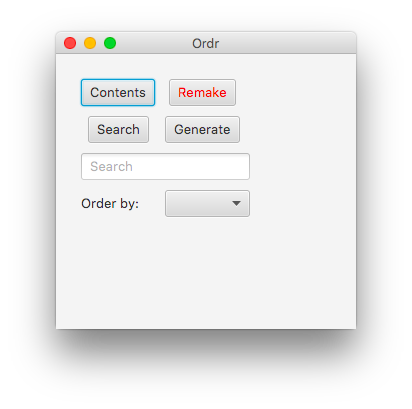
\includegraphics[scale=0.5]{MainMenu}
	\caption{Main Menu}
	\label{mm}
\end{figure}
This is the main menu, where every other function can be called.
\begin{figure}[H]
	\centering
	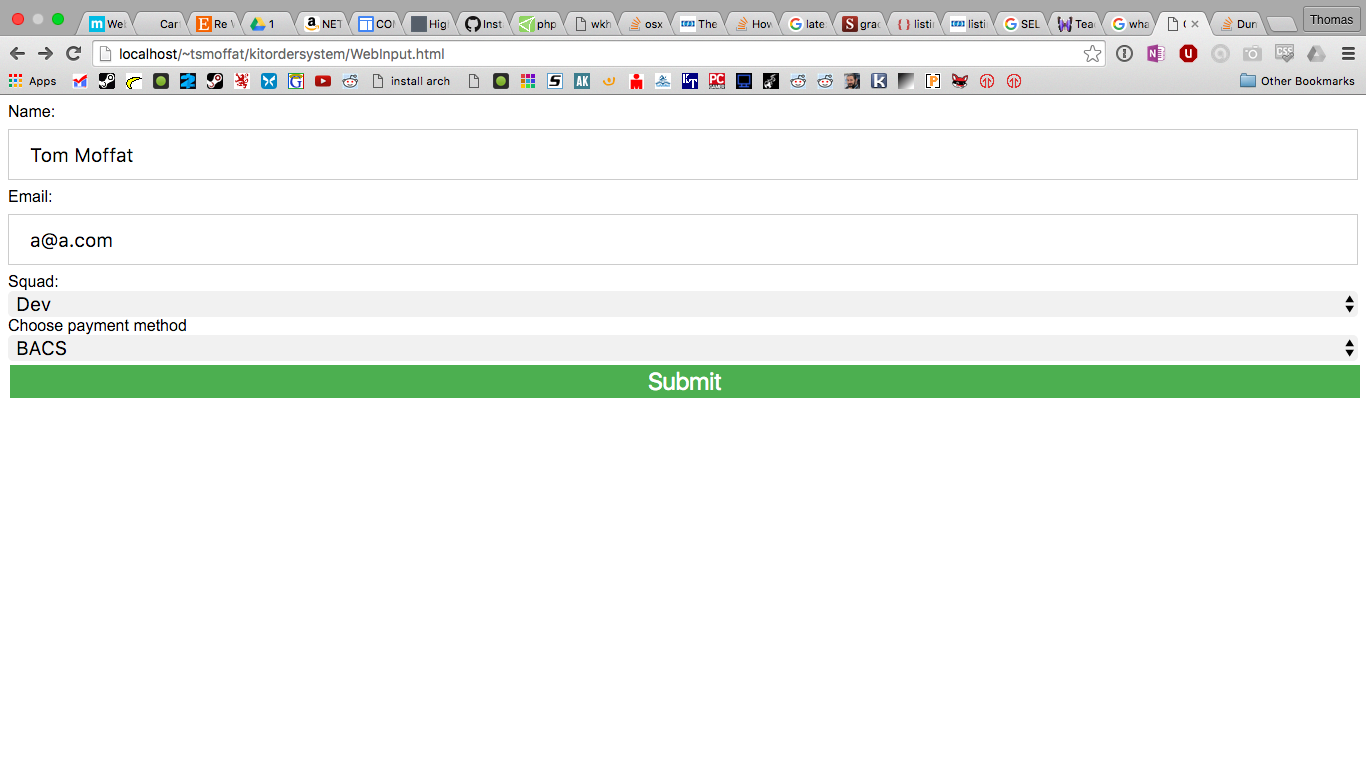
\includegraphics[width=\linewidth]{CustomerForm}
	\caption{Order Form}
	\label{of}
\end{figure}
This is the form where the customer inputs their details. When the submit button is clicked it is inserted into the database.
\begin{figure}[H]
	\centering
	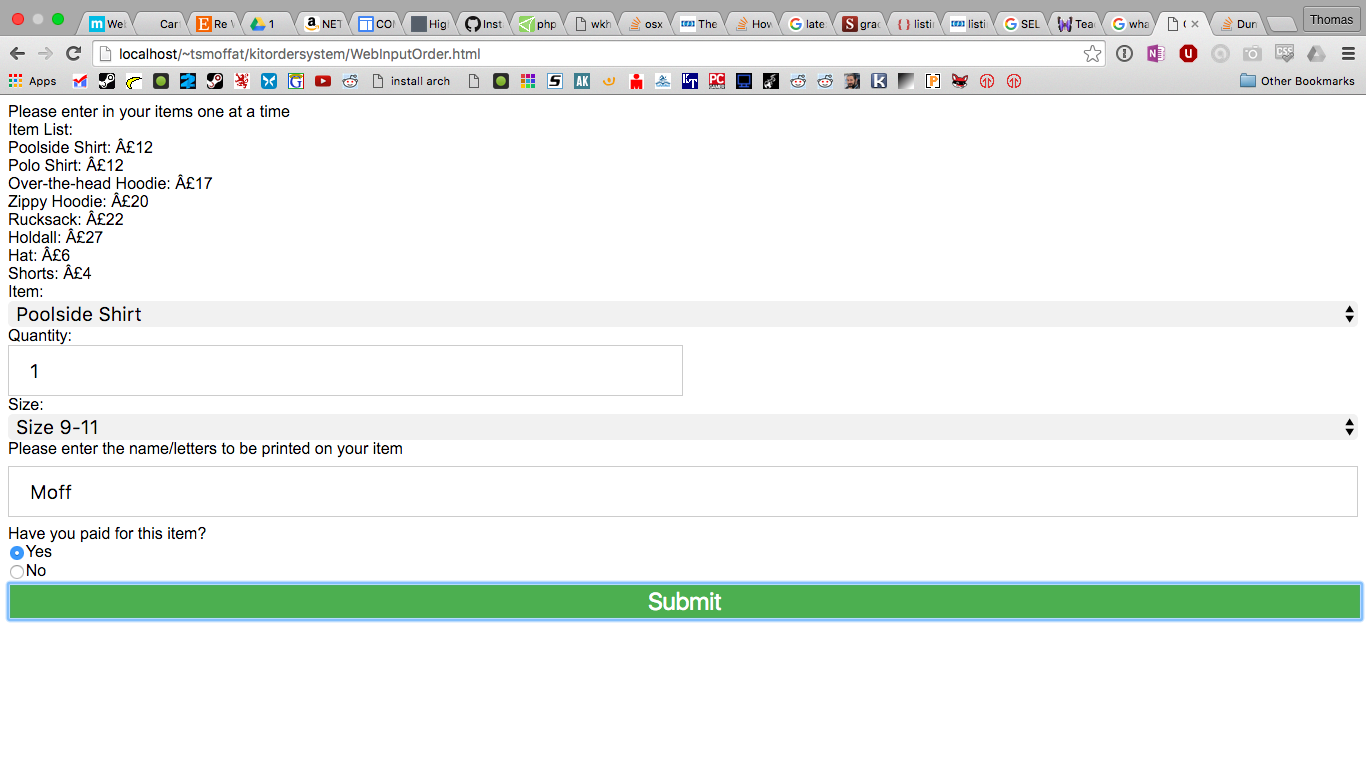
\includegraphics[width=\linewidth]{OrderForm}
	\caption{Customer Form}
	\label{cf}
\end{figure}
This is the form where the customers input their orders. When the submit button is clicked the order details are passed to the database.
\begin{figure}[H]
	\centering
	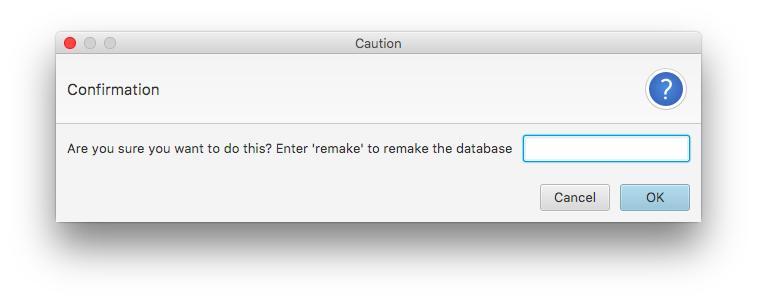
\includegraphics[scale=0.5]{ConfirmBox}
	\caption{Confirmation Box}
	\label{cb}
\end{figure}
This is the confirmation box that appears when the Kit Coordinator clicks Remake, which makes sure they do actually want to remake the database
\begin{figure}[H]
	\centering
	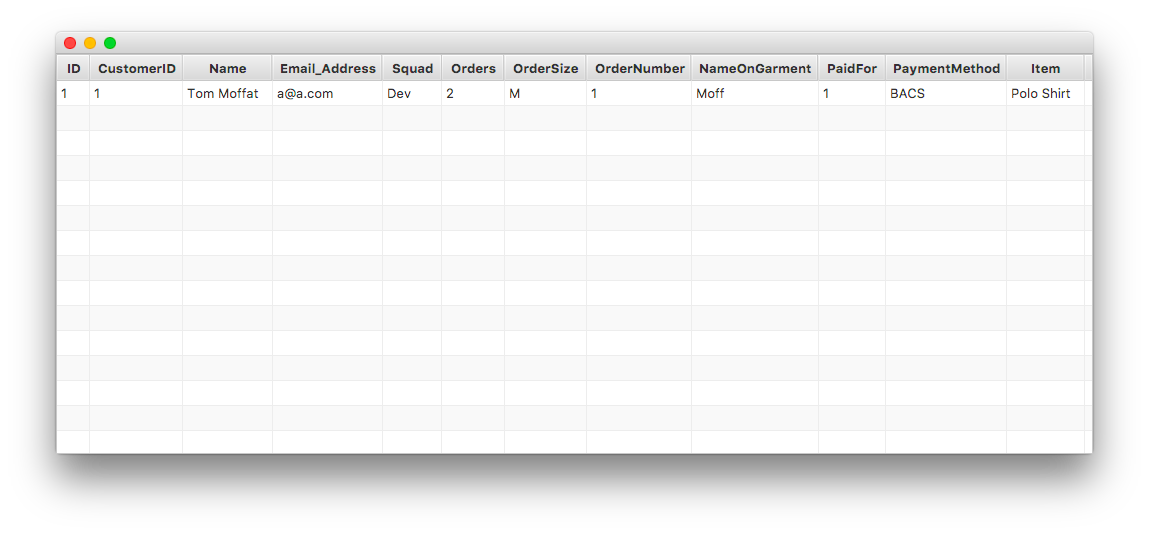
\includegraphics[width=\linewidth]{OutputTable}
	\caption{The table output when clicking on contents or search}
	\label{ot}
\end{figure}
\begin{figure}[H]
	\centering
	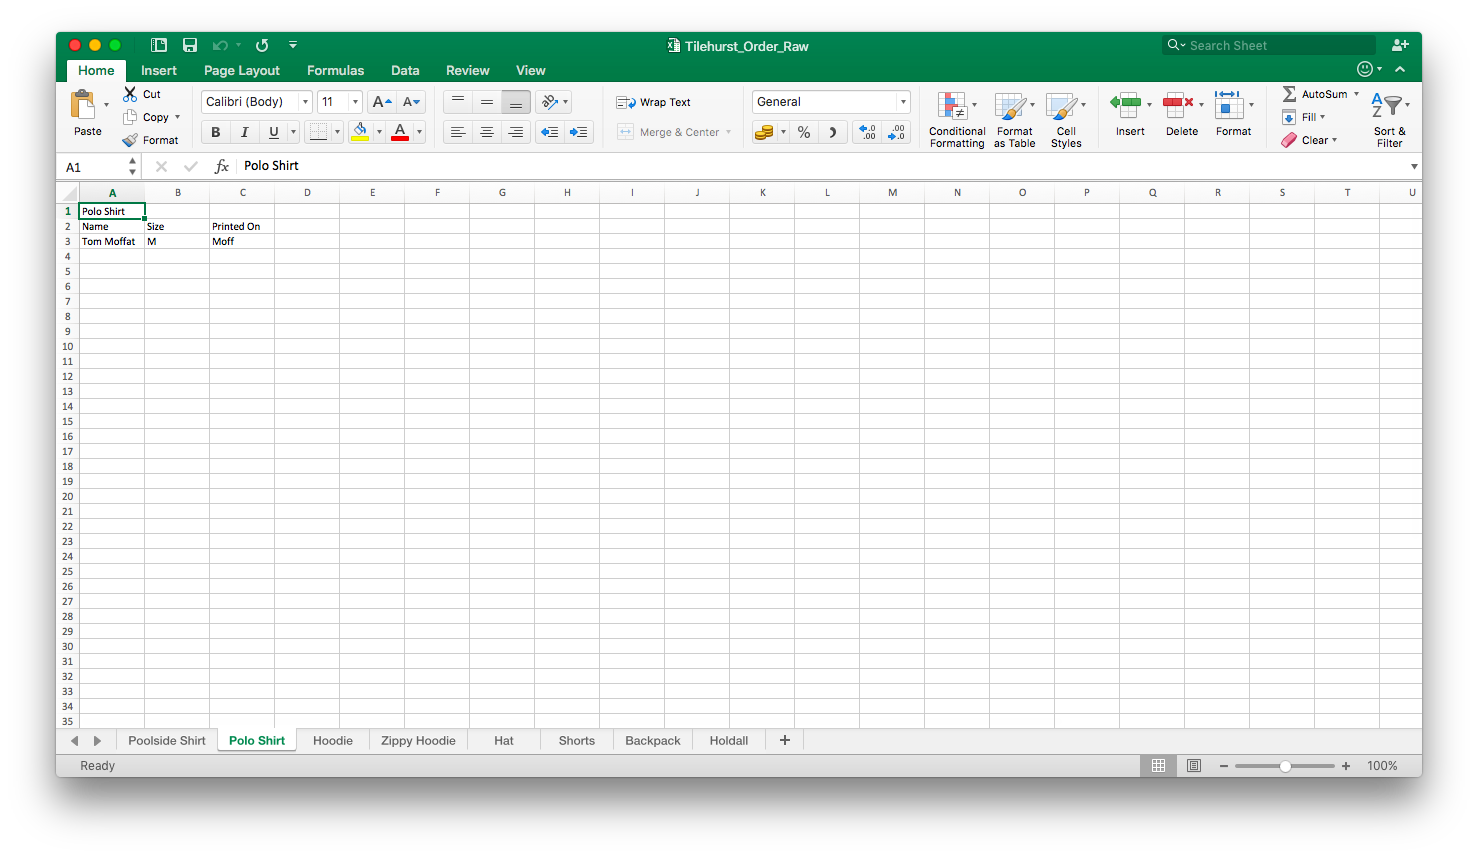
\includegraphics[width=\linewidth]{OutputExcel}
	\caption{The Excel Spreadsheet generated when Generate is clicked that will be sent off to the printer}
	\label{oe}
\end{figure}
\begin{figure}
	\centering
	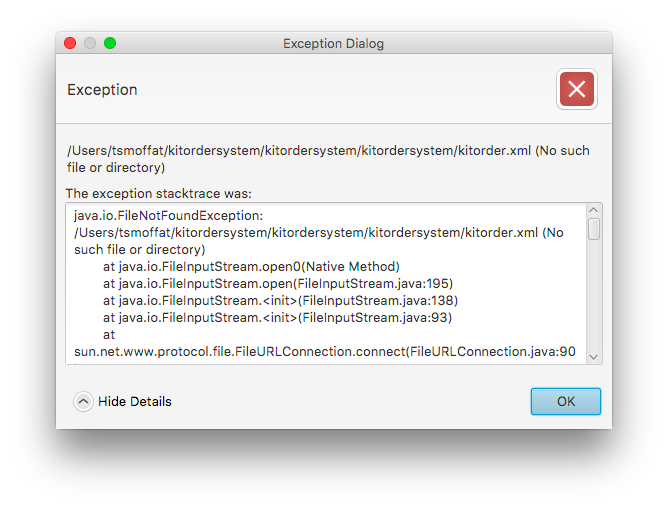
\includegraphics[scale=0.5]{JavaUpdatedError}
	\caption{The error dialog that appears when the program hits an exception}
	\label{jue}	
\end{figure}

\end{document}